%%%%%%%%%%%%%%%%%%%%%%%%%%%%%%%%%%%%%%%%%
% Programming/Coding Assignment
% LaTeX Template
%
% This template has been downloaded from:
% http://www.latextemplates.com
%
% Original author:
% Ted Pavlic (http://www.tedpavlic.com)
%
% Note:
% The \lipsum[#] commands throughout this template generate dummy text
% to fill the template out. These commands should all be removed when 
% writing assignment content.
%
% This template uses a Perl script as an example snippet of code, most other
% languages are also usable. Configure them in the "CODE INCLUSION 
% CONFIGURATION" section.
%
%%%%%%%%%%%%%%%%%%%%%%%%%%%%%%%%%%%%%%%%%

%----------------------------------------------------------------------------------------
%	PACKAGES AND OTHER DOCUMENT CONFIGURATIONS
%----------------------------------------------------------------------------------------

\documentclass{article}

\usepackage{fancyhdr} % Required for custom headers
\usepackage{lastpage} % Required to determine the last page for the footer
\usepackage{extramarks} % Required for headers and footers
\usepackage[usenames,dvipsnames]{color} % Required for custom colors
\usepackage{graphicx} % Required to insert images
\usepackage{listings} % Required for insertion of code
\usepackage{courier} % Required for the courier font
\usepackage{lipsum} % Used for inserting dummy 'Lorem ipsum' text into the template
\usepackage{setspace}
\usepackage{color}
\usepackage{comment}
\usepackage{caption}

\usepackage{hyperref}
\usepackage{natbib}
\usepackage{underscore}
\usepackage{subfigure}


\hypersetup{
    colorlinks=true,
    linkcolor=blue,
    filecolor=magenta,      
    urlcolor=cyan,
    breaklinks=true
}

%\usepackage[]{algorithm2e}
\usepackage{pdfpages}




%For python inclusion (http://widerin.org/blog/syntax-highlighting-for-python-scripts-in-latex-documents)
\definecolor{Code}{rgb}{0,0,0}
\definecolor{Decorators}{rgb}{0.5,0.5,0.5}
\definecolor{Numbers}{rgb}{0.5,0,0}
\definecolor{MatchingBrackets}{rgb}{0.25,0.5,0.5}
\definecolor{Keywords}{rgb}{0,0,1}
\definecolor{self}{rgb}{0,0,0}
\definecolor{Strings}{rgb}{0,0.63,0}
\definecolor{Comments}{rgb}{0,0.63,1}
\definecolor{Backquotes}{rgb}{0,0,0}
\definecolor{Classname}{rgb}{0,0,0}
\definecolor{FunctionName}{rgb}{0,0,0}
\definecolor{Operators}{rgb}{0,0,0}
\definecolor{Background}{rgb}{0.98,0.98,0.98}

% Margins
\topmargin=-0.45in
\evensidemargin=0in
\oddsidemargin=0in
\textwidth=6.5in
\textheight=9.0in
\headsep=0.25in

\linespread{1.1} % Line spacing

% Set up the header and footer
\pagestyle{fancy}
\lhead{\hmwkAuthorName} % Top left header
%\chead{\hmwkClass\ (\hmwkClassInstructor\ \hmwkClassTime): \hmwkTitle} % Top center head
\chead{\hmwkClass\ (\hmwkClassInstructor): \hmwkTitle} % Top center head
\rhead{\firstxmark} % Top right header
\lfoot{\lastxmark} % Bottom left footer
\cfoot{} % Bottom center footer
\rfoot{Page\ \thepage\ of\ \protect\pageref{LastPage}} % Bottom right footer
\renewcommand\headrulewidth{0.4pt} % Size of the header rule
\renewcommand\footrulewidth{0.4pt} % Size of the footer rule

\setlength\parindent{0pt} % Removes all indentation from paragraphs

%----------------------------------------------------------------------------------------
%	CODE INCLUSION CONFIGURATION
%----------------------------------------------------------------------------------------

\definecolor{MyDarkGreen}{rgb}{0.0,0.4,0.0} % This is the color used for comments
\lstloadlanguages{Perl} % Load Perl syntax for listings, for a list of other languages supported see: ftp://ftp.tex.ac.uk/tex-archive/macros/latex/contrib/listings/listings.pdf
\lstset{language=Perl, % Use Perl in this example
        frame=single, % Single frame around code
        basicstyle=\small\ttfamily, % Use small true type font
        keywordstyle=[1]\color{Blue}\bf, % Perl functions bold and blue
        keywordstyle=[2]\color{Purple}, % Perl function arguments purple
        keywordstyle=[3]\color{Blue}\underbar, % Custom functions underlined and blue
        identifierstyle=, % Nothing special about identifiers                                         
        commentstyle=\usefont{T1}{pcr}{m}{sl}\color{MyDarkGreen}\small, % Comments small dark green courier font
        stringstyle=\color{Purple}, % Strings are purple
        showstringspaces=false, % Don't put marks in string spaces
        tabsize=5, % 5 spaces per tab
        %
        % Put standard Perl functions not included in the default language here
        morekeywords={rand},
        %
        % Put Perl function parameters here
        morekeywords=[2]{on, off, interp},
        %
        % Put user defined functions here
        morekeywords=[3]{test},
       	%
        morecomment=[l][\color{Blue}]{...}, % Line continuation (...) like blue comment
        numbers=left, % Line numbers on left
        firstnumber=1, % Line numbers start with line 1
        numberstyle=\tiny\color{Blue}, % Line numbers are blue and small
        stepnumber=5 % Line numbers go in steps of 5
}

% Creates a new command to include a perl script, the first parameter is the filename of the script (without .pl), the second parameter is the caption
\newcommand{\perlscript}[2]{
\begin{itemize}
\item[]\lstinputlisting[caption=#2,label=#1]{#1.pl}
\end{itemize}
}


%----------------------------------------------------------------------------------------
%	DOCUMENT STRUCTURE COMMANDS
%	Skip this unless you know what you're doing
%----------------------------------------------------------------------------------------

% Header and footer for when a page split occurs within a problem environment
\newcommand{\enterProblemHeader}[1]{
\nobreak\extramarks{#1}{#1 continued on next page\ldots}\nobreak
\nobreak\extramarks{#1 (continued)}{#1 continued on next page\ldots}\nobreak
}

% Header and footer for when a page split occurs between problem environments
\newcommand{\exitProblemHeader}[1]{
\nobreak\extramarks{#1 (continued)}{#1 continued on next page\ldots}\nobreak
\nobreak\extramarks{#1}{}\nobreak
}

\setcounter{secnumdepth}{0} % Removes default section numbers
\newcounter{homeworkProblemCounter} % Creates a counter to keep track of the number of problems

\newcommand{\homeworkProblemName}{}
\newenvironment{homeworkProblem}[1][Problem \arabic{homeworkProblemCounter}]{ % Makes a new environment called homeworkProblem which takes 1 argument (custom name) but the default is "Problem #"
\stepcounter{homeworkProblemCounter} % Increase counter for number of problems
\renewcommand{\homeworkProblemName}{#1} % Assign \homeworkProblemName the name of the problem
\section{\homeworkProblemName} % Make a section in the document with the custom problem count
\enterProblemHeader{\homeworkProblemName} % Header and footer within the environment
}{
\exitProblemHeader{\homeworkProblemName} % Header and footer after the environment
}

\newcommand{\problemAnswer}[1]{ % Defines the problem answer command with the content as the only argument
\noindent\framebox[\columnwidth][c]{\begin{minipage}{0.98\columnwidth}#1\end{minipage}} % Makes the box around the problem answer and puts the content inside
}

\newcommand{\homeworkSectionName}{}
\newenvironment{homeworkSection}[1]{ % New environment for sections within homework problems, takes 1 argument - the name of the section
\renewcommand{\homeworkSectionName}{#1} % Assign \homeworkSectionName to the name of the section from the environment argument
\subsection{\homeworkSectionName} % Make a subsection with the custom name of the subsection
\enterProblemHeader{\homeworkProblemName\ [\homeworkSectionName]} % Header and footer within the environment
}{
\enterProblemHeader{\homeworkProblemName} % Header and footer after the environment
}

%----------------------------------------------------------------------------------------
%	NAME AND CLASS SECTION
%----------------------------------------------------------------------------------------

\newcommand{\hmwkTitle}{Assignment\ \#7 } % Assignment title
%\newcommand{\hmwkDueDate}{Monday,\ January\ 1,\ 2012} % Due date
\newcommand{\hmwkClass}{Introduction to Web Science} % Course/class
%\newcommand{\hmwkClassTime}{10:30am} % Class/lecture time
\newcommand{\hmwkClassInstructor}{Dr. Nelson} % Teacher/lecturer
\newcommand{\hmwkAuthorName}{Alexander Nwala} % Your name

%----------------------------------------------------------------------------------------
%	TITLE PAGE
%----------------------------------------------------------------------------------------

\title{
\vspace{2in}
\textmd{\textbf{\hmwkClass:\ \hmwkTitle}}\\
%\normalsize\vspace{0.1in}\small{Due\ on\ \hmwkDueDate}\\
%\vspace{0.1in}\large{\textit{\hmwkClassInstructor\ \hmwkClassTime}}
\vspace{0.1in}\large{\textit{\hmwkClassInstructor}}
\vspace{3in}
}

\author{\textbf{\hmwkAuthorName}}
\date{Thursday, November 6, 2014} % Insert date here if you want it to appear below your name

%----------------------------------------------------------------------------------------

\begin{document}

\maketitle



%----------------------------------------------------------------------------------------
%	TABLE OF CONTENTS
%----------------------------------------------------------------------------------------

%\setcounter{tocdepth}{1} % Uncomment this line if you don't want subsections listed in the ToC

\newpage
\tableofcontents
\newpage

%----------------------------------------------------------------------------------------
%	PROBLEM 1
%----------------------------------------------------------------------------------------

% To have just one problem per page, simply put a \clearpage after each problem

\begin{homeworkProblem}

Using D3, create a graph of the Karate club before and after
the split.\\

- Weight the edges with the data from:\\
\url{http://vlado.fmf.uni-lj.si/pub/networks/data/ucinet/
zachary.dat}\\

- Have the transition from before/after the split occur on a mouse
click.


%\problemAnswer
%{
    \begin{verbatim}\end{verbatim}
    \textbf{SOLUTION 1}\\

    With the use of D3.js (a JavaScript library for manipulating documents based on data) \cite{d3}, and the Force-Directed Graph template for undirected graphs (\url{http://bl.ocks.org/mbostock/4062045}), the following solution was achieved.\\

    The solution for this problem is outlined by the following steps:
    \begin{enumerate}

    \item \textbf{Convert the Karate club graph to json:} With the use of BeautifulSoup \cite{BeautifulSoup}, as outlined in Listing 1, the Karate club graph, karate.GraphML was converted to karateClubGraph.json.
    \lstinputlisting[breaklines=true, caption=Convert karate.GraphML to karateClubGraph.json]{convertGraphSnippet.py}

    \item \textbf{Color code graph based on before/after split:} In karateClubGraph.json, every node was given the same ``color'' attribute, but a different color based on it's ``faction'' attibute as outlined below

    \begin{verbatim}
    ...
     {"name": "Mr Hi", "faction": 1, "color": 1 },
     {"name": "2", "faction": 1, "color": 1 },
     {"name": "3", "faction": 1, "color": 1 },
     {"name": "4", "faction": 1, "color": 1 },
     {"name": "5", "faction": 1, "color": 1 },
     {"name": "6", "faction": 1, "color": 1 },
     {"name": "7", "faction": 1, "color": 1 },
     {"name": "8", "faction": 1, "color": 1 },
     {"name": "9", "faction": 2, "color": 1 },
     {"name": "10", "faction": 2, "color": 1 },
     ...
    \end{verbatim}

    \item \textbf{Toggle node color on click:} As shown in Listing 2. All nodes have been wired to the on click event. This means when any node is clicked, the function specialNodeClick, is called. And this function simply toggles the fill color of the nodes from the static color to the colors representing the different factions.

    \lstinputlisting[breaklines=true, caption=Toggle node color]{onClickSnippet.js}
   
    \end{enumerate}
    
    \textbf{CONCLUSION 1}\\


    The result (Figure 1) of the foregoing operations can be seen at 
    \url{http://www.cs.odu.edu/\~anwala/files/temp/karateClub.html}

    \begin{figure}[h!]

        \caption{Karate Club Graph}
        \subfigure[Before Split]{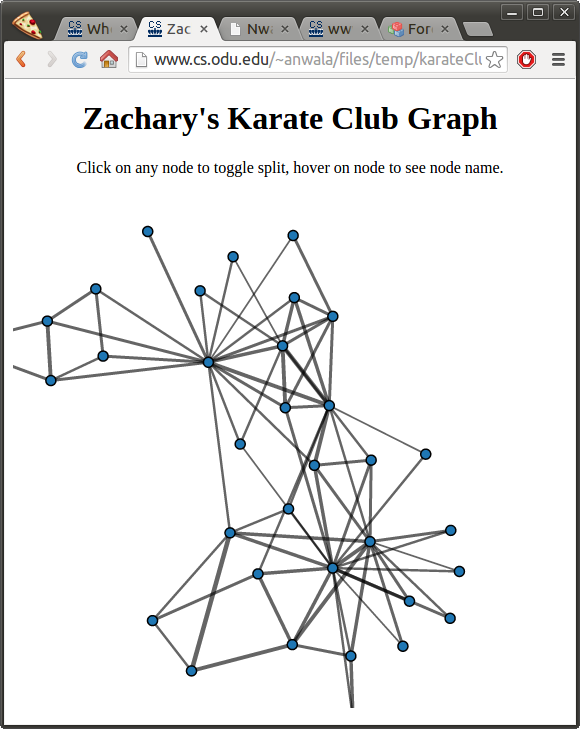
\includegraphics[width=.50\textwidth]{../figures/karateClubBeforeSplit.png}}
        \subfigure[After Split]{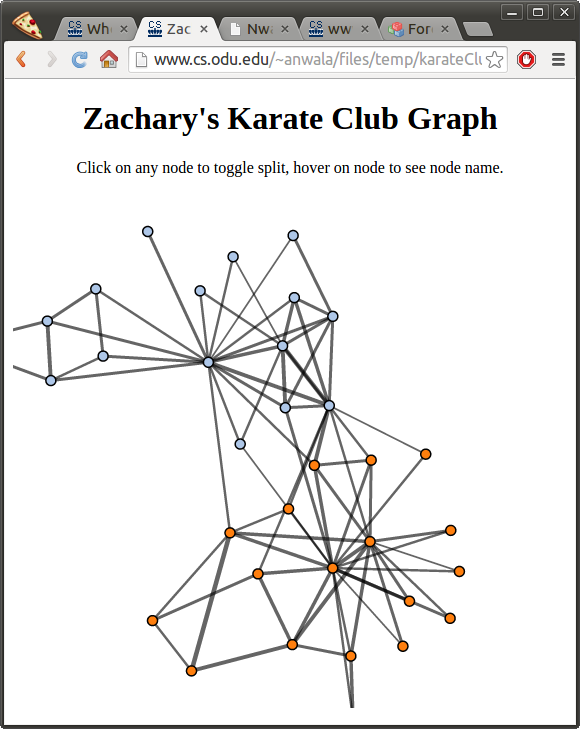
\includegraphics[width=.50\textwidth]{../figures/karateClubAfterSplit.png}}

    \end{figure}

%}



\end{homeworkProblem}

%----------------------------------------------------------------------------------------
%	PROBLEM 2
%----------------------------------------------------------------------------------------
\begin{homeworkProblem}

Use D3 to create a who-follows-whom graph of your Twitter
account.  Use my twitter account (``@phonedude_mln'') if you do not
have an interesting number of followers.  Attractiveness of the 
graph counts!\\

Note: for getting GitHub to serve HTML (and other media types), see:\\

http://stackoverflow.com/questions/6551446/can-i-run-html
-files-directly-from-github-instead-of-just-viewing-their-source

\begin{verbatim}\end{verbatim}
\textbf{SOLUTION 2}\\

With the use of D3.js (a JavaScript library for manipulating documents based on data) \cite{d3}, and the Force-Directed Graph template for directed graphs (\url{http://bl.ocks.org/mbostock/1153292}), following solution was achieved.\\

The solution for this problem is outlined by the following steps:
\begin{enumerate}

\item \textbf{Develop an algorithm to get the followers of followers:} In order to get the followers of followers across a variable degree, I derived the iterative algorithm (gen) presented in below:

\begin{verbatim}
Input: 
    twitterScreenName (s)
    maximumFollowerCount (m)
    maximumDegreeOfGraph (d)
    graphOutputFile (O)
Output:
    A graph file O, with the following format:

    <1st degree follower 1>+...+
        <2nd degree follower 1>+...+
            <3rd degree follower 1>+...+
                ...<nth degree follower 1>+
                   <nth degree follower 2>+
                   ...
                   <nth degree follower n>+
            <3rd degree follower 2>
            ...
            <3rd degree follower n>
        <2nd degree follower 2>
        ...
        <2nd degree follower n>
    <1st degree follower 2>+
    ...
    <1st degree follower n>+






procedure gen( s, m, d )
    while( end = False )

        if( O is empty ) then
            followersList = getFollowersFromTwitter(s, m);
            O.write( followersList );
        else:
            follower = 
            getFollowerWithMinimumPlusCountAndWithinDegree(followersList, d);

            followersList = getFollowersFromTwitter(follower, d);
            O.write( followersList );

            if( all followers have been explored ) then
                end = True;
            endif
        endif
end

procedure getFollowersFromTwitter( userId, countOfFollowersToReturn )
    n = countOfFollowersToReturn;
    if( operation on userId is authorized ) then
        listOfFollowers = <follower1, follower2,..., follower(n)>;
    else
        listOfFollowers = <>;
    endif

    return listOfFollowers;
end

getFollowerWithMinimumPlusCountAndWithinDegree( listOfFollowers, d )
    
    follower = None;
    minimumPlus = Infinity;

    foreach follower in listOfFollowers:
        plusCount, tabCount = getPlusCountAndTabCount(follower);

        if( plusCount != 0 and plusCount < d ) then
            if( plusCount < minimumPlus and tabCount < d ) then
                minimumPlus = plusCount;
                item = follower;
            endif
        endif
    endfor
end

\end{verbatim}

The implementation of gen(), is outlined in Listing 3.
\lstinputlisting[breaklines=true, caption=Get followers of followers: gen()]{getFoFSnippet.py}

\item \textbf{Convert gen()'s output O to a links file:} This was achieved by a python script as shown in Listing 4.

\lstinputlisting[breaklines=true, caption=Generate graph file]{generateGraphFileSnippet.py}

\item \textbf{Visualize graph:} With the use of the graph template at \url{http://bl.ocks.org/mbostock/1153292}, I replaced the default data in the JavaScript file with the output of gen() as outlined in Listing 5.

\lstinputlisting[breaklines=true, caption=Who follows who graph file]{whoFollowsWhoSnippet.js}

\end{enumerate}

\textbf{CONCLUSION 2}\\

The result of running gen() (Figure 2.) can be seen at\\
\url{http://www.cs.odu.edu/~anwala/files/temp/whosFollowingWho.html}


\begin{figure}
    \caption{Who follows who}
    \subfigure[Who follows who]{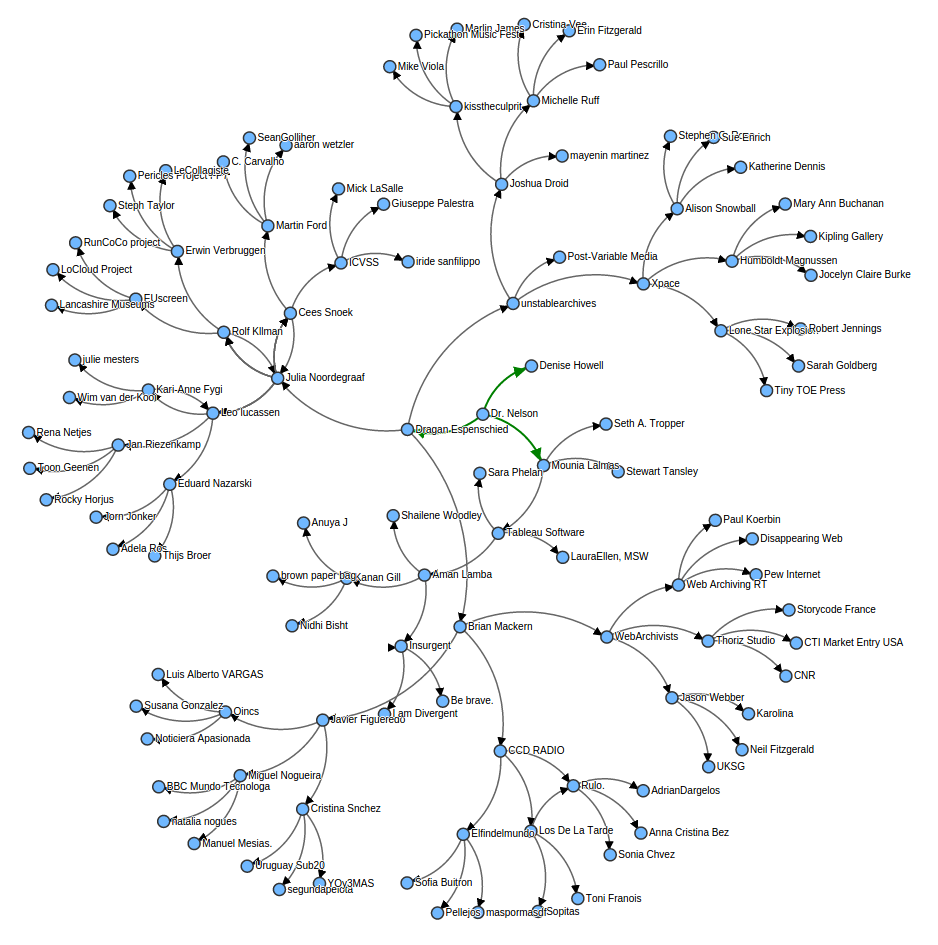
\includegraphics[width=\textwidth]{../figures/whoFollowsWho.png}}
\end{figure}

\end{homeworkProblem}

\begin{verbatim}





















\end{verbatim}
\bibliographystyle{plain}
\bibliography{A7bibFile}

%----------------------------------------------------------------------------------------

\end{document}